\section{Baseline Architecture Details}
\label{sec:baseline-architectures}

\subsection{Battling Track Baselines}

PokéChamp \cite{karten2025pok} and Metamon \cite{grigsby2025human} form the foundation for our Battling Track baselines. Both projects were significantly upgraded to improve their competitive performance and serve as extensible starter points for future work. All of these changes are open-source and detailed information is available via the \href{https://pokeagentchallenge.com}{PokéAgent Challenge Resources Page}. This section provides a high-level introduction and summarizes key improvements.

\subsubsection{PokéChamp}

PokéChamp combines large language models with minimax search for competitive battling. The system converts game state to text via a game engine interface, then uses an LLM to evaluate positions through an approximate state transition heuristic. This enables strategic lookahead without requiring explicit reward signals or training data.

\begin{figure}[h]
    \centering
    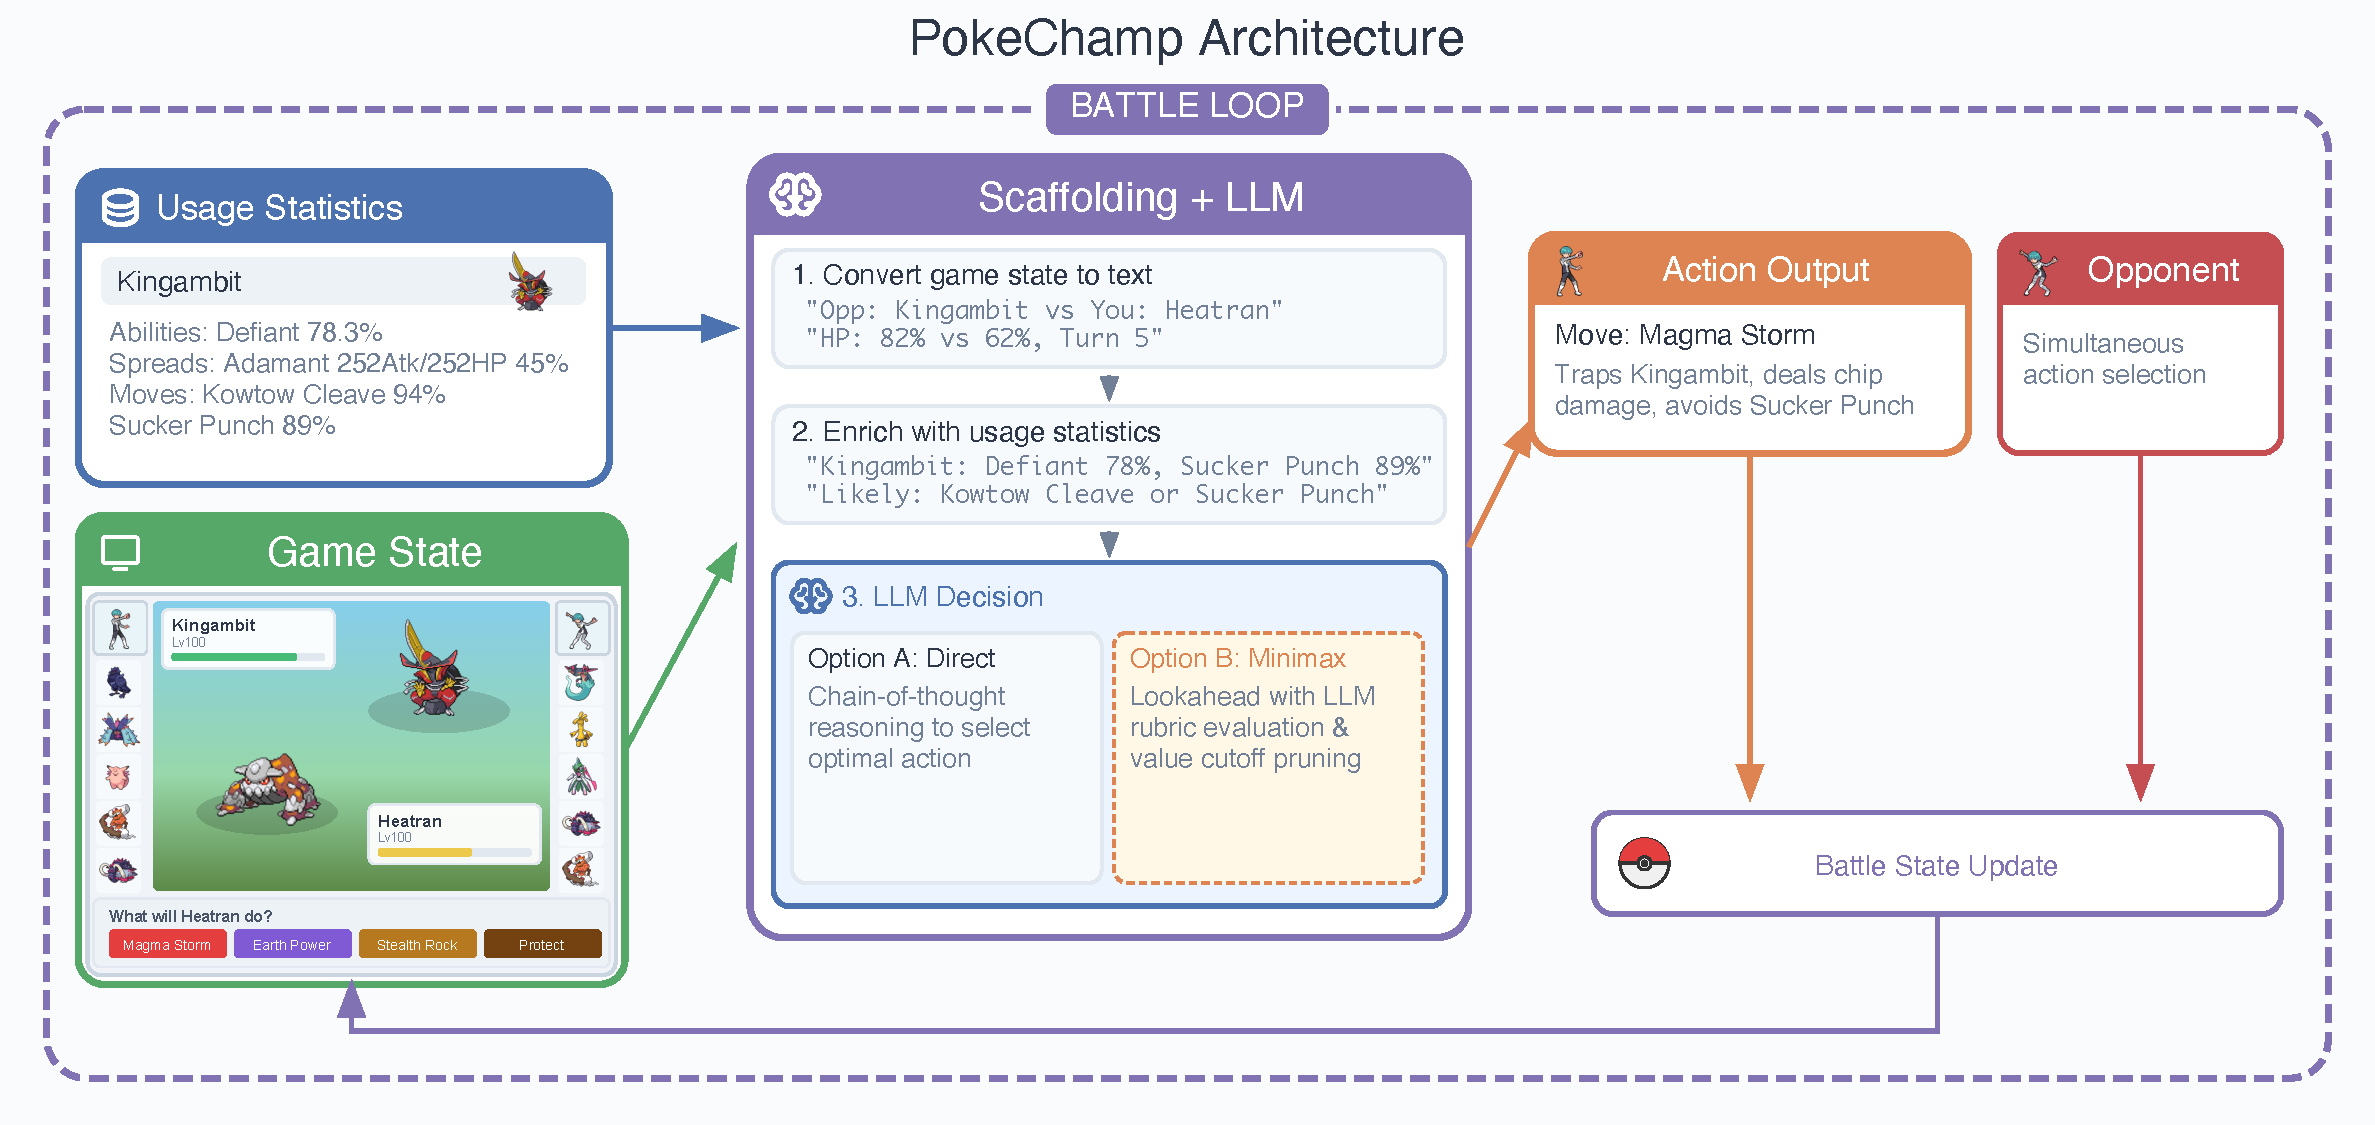
\includegraphics[width=.95\linewidth]{figures/pokechamp_architecture.pdf}
    \caption{\textbf{PokeChamp Architecture.} Within the battle loop, two data sources feed into the LLM pipeline: (1)~historical usage statistics from Smogon (left top), providing probability distributions over abilities, EV spreads, and moves for each species; and (2)~the current game state from Pokémon Showdown (left bottom). The Text Conversion + LLM module (center) converts game state to structured text, enriches it with usage statistics for opponent prediction, and performs LLM inference to select actions. The chosen move executes and updates the game state for the next turn.}
    \label{fig:pokechamp}
\end{figure}

\subsubsection{Metamon}

Metamon converts Showdown's replay archives into an opportunity to study offline RL \cite{levine2020offline} at scale in a complex domain. Its baselines embrace the complexity and partial observability of Pokémon by training Transformer policies with model-free off-policy RL updates \cite{grigsbyamago}. Further improvements beyond the human demonstration dataset are driven by a large-scale ``replay across experiments'' \cite{tirumalareplay} loop in which the project continuously expands a central repository of self-play trajectories and policies (Figure \ref{fig:metamon}). As of the launch of the PokéAgent Challenge, the training dataset exceeds $20$M battles and has produced $30$ meaningfully distinct policies at various skill levels. Metamon training runs are expensive by academic standards and each iteration may have several axes of improvement (datasets, architectures, RL details). As a result, its agent releases are given somewhat arbitrary names (LLM-style) that are excluded from results like Figures \ref{fig:track1_baselines} and \ref{fig:neurips_track1_main_text} but are available in PokéAgent Challenge resources. Table \ref{tab:metamon_baselines} defines a short list that are relevant to the NeurIPS competition results (Appendix \ref{sec:track1-full-results}) or referenced by particpant writeups in (Appendix \ref{sec:participant-methodologies}).

\begin{figure}[h!]
    \centering
    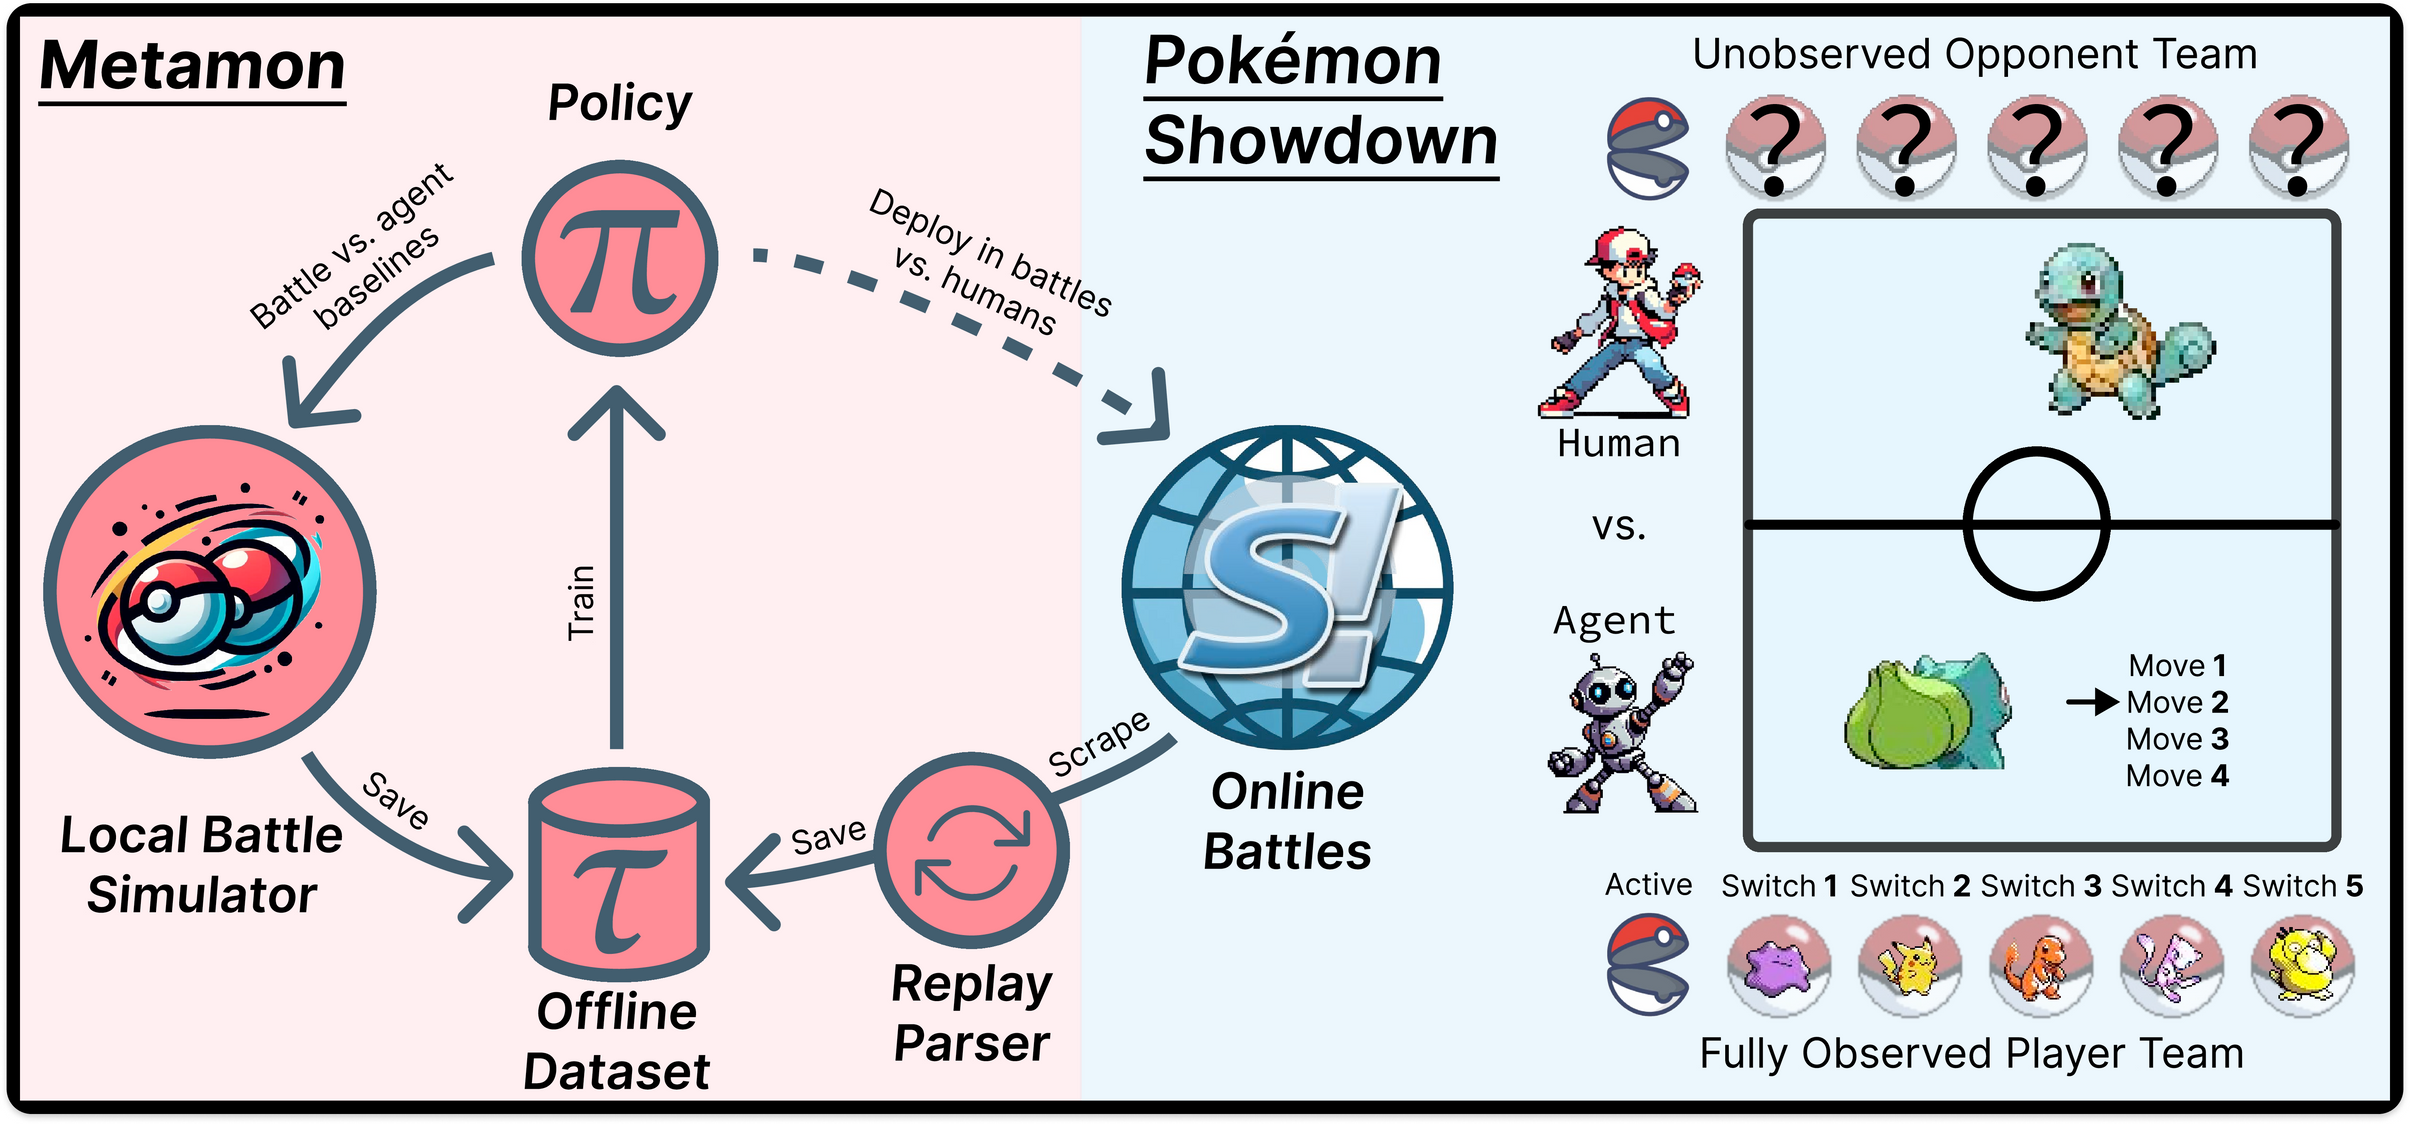
\includegraphics[width=.80\linewidth]{figures/metamon_training.png}
    \caption{\textbf{Metamon Training Pipeline.} Metamon trains RL agents on large datasets of self-play battles and human demonstrations ``reconstructed'' from replays gathered from Pokémon Showdown. Figure reproduced from \citet{grigsby2025human}.}
    \label{fig:metamon}
\end{figure}



\begin{table}[htbp]
\centering
\renewcommand{\arraystretch}{1.3} 
\resizebox{.95\textwidth}{!}{%
\begin{tabular}{l c c p{10cm} c c c c c}
\toprule
\multirow{2}{*}{\textbf{Model}} & \multirow{2}{*}{\textbf{Size}} & \multirow{2}{*}{\textbf{Date}} & \multirow{2}{*}{\textbf{Description}} & \multicolumn{5}{c}{\textbf{Human Ladder Ratings (GXE)}} \\
\cmidrule(lr){5-9}
& & & & \textbf{G1} & \textbf{G2} & \textbf{G3} & \textbf{G4} & \textbf{G9} \\
\midrule
\texttt{SyntheticRLV2} & 200M & Sep 2024 & The best (public) Gen 1 OU policy during the NeurIPS competition, and therefore the basis of many of the qualifying submissions (Appendix \ref{sec:participant-methodologies}). & 77\% & 68\% & 64\% & 66\% & -- \\
\addlinespace
\texttt{Abra} & 57M & Jul 2025 & The best (public) Gen 9 OU policy during the NeurIPS competition, and therefore the basis of many of the qualifying submissions (Appendix \ref{sec:participant-methodologies}). & -- & -- & -- & -- & 50\% \\
\addlinespace
\texttt{Kadabra3} & 57M & Sep 2025 & The best policy to participate in the NeurIPS competition as an organizer baseline (rank \#1 in the Gen 1 OU qualifier and \#2 in Gen 9 OU). & 80\% & -- & -- & -- & 64\% \\
\addlinespace
\texttt{Kakuna} & 142M & Dec 2025 & The best metamon model as of the launch of the PokéAgent Challenge (with results appearing in Fig. \ref{fig:track1_baselines}). & 82\% & 70\% & 63\% & 64\% & 71\% \\
\bottomrule
\end{tabular}%
}
\vspace{1mm}
\caption{Metamon baselines referenced in Appendix results, and their estimated performance against human players. ``G1'' $\rightarrow$ ``Gen 1 OU''.}
\label{tab:metamon_baselines}
\end{table}



The most notable improvement made to Metamon for the PokéAgent Challenge was its expansion to support the Gen 9 OU ruleset, which created the opportunity for RL and LLM baselines to compete directly. Gen 9 OU has a significantly larger state space (Appendix \ref{sec:state-space-derivation}) than the rulesets from the original work, and it was an open question whether model-free RL would generalize to this more complex game. Today, Metamon is at least as competitive against human players in Gen 9 OU as earlier generations (Table \ref{tab:metamon_baselines}), though its performance in Gen 1 OU remains an outlier. 

\subsection{Speedrunning Track Baselines}
\label{sec:pokeagent-architecture}

The \pokeagent starter kit implements a \textbf{multi-agent orchestration system} that successfully completed Pokémon Emerald. The architecture distinguishes between two types of capabilities: \textit{MCP tools} for low-level game interaction and \textit{sub-agents} for high-level reasoning. A central orchestrator coordinates these components, dispatching to specialized sub-agents based on game context while using MCP tools for direct game control.

\begin{figure}[h]
    \centering
    
\includegraphics[width=\linewidth]{figures/pokeagent_architecture.pdf}
    \caption{\textbf{\pokeagent Multi-Agent Architecture.} The orchestrator coordinates sub-agents and MCP tools to play the game. Data flows left-to-right from the GBA emulator (game frames, parsed state) through the Orchestrator (context management, sub-agent dispatch, stuck detection), which invokes either MCP tools (pathfinding, button inputs, knowledge retrieval) for direct game control or specialized sub-agents (battle agent, reflection agent, verification agent, gym puzzle agent) for complex reasoning tasks. A feedback loop returns sub-agent outputs and tool results to inform subsequent decisions.}
    \label{fig:pokeagent_arch}
\end{figure}

\paragraph{Orchestrator.} The flagship harness implements a central orchestrator that coordinates all sub-agents and tool calls. Upon initialization, the orchestrator invokes a \textit{planning sub-agent} to generate a high-level route covering story progression, team building objectives (training, catching, item acquisition), and resource management (Pokémon Center visits). This loose plan maintains long-term coherence while allowing ad-hoc objective creation during gameplay. The orchestrator dispatches to specialized sub-agents based on context: the \textit{battle sub-agent} handles combat decisions, the \textit{reflection sub-agent} analyzes stuck states, and the \textit{verification sub-agent} checks objective completion to prevent premature advancement.

The system exposes two categories of capabilities to the orchestrator:

\paragraph{MCP Tools.} Low-level game interaction via HTTP endpoints:
\begin{itemize}
    \item \textbf{Game Control}: \texttt{get\_game\_state}, \texttt{press\_buttons}, and \texttt{navigate\_to} (A* pathfinding with variance options for obstacle handling)
    \item \textbf{Knowledge Retrieval}: Persistent memory system storing discoveries (locations, NPCs, items, strategies) with importance-weighted retrieval.
    \item \textbf{Objective Management}: Three parallel objective sequences---\textit{story} (main narrative), \textit{battling} (team building), and \textit{dynamics} (agent-created adaptive goals)---enabling balanced progress across game dimensions
\end{itemize}

\paragraph{Sub-Agents.} Specialized reasoning modules invoked by the orchestrator:
\begin{itemize}
    \item \textbf{Battle Sub-Agent}: Handles combat decisions including move selection, switching, and item usage based on type matchups and team state
    \item \textbf{Reflection Sub-Agent}: Analyzes stuck states by comparing current situation against ground truth sources (porymap data, knowledge base) to diagnose navigation failures
    \item \textbf{Verification Sub-Agent}: Independently checks whether objectives are truly complete, preventing the orchestrator from advancing when the main agent incorrectly believes a task is finished
    \item \textbf{Gym Puzzle Sub-Agent}: Specialized reasoning for gym-specific puzzles requiring spatial planning (e.g., Mauville's electric barriers, Lavaridge's floor tiles)
\end{itemize}

Interestingly, wiki access via the knowledge retrieval tool sometimes degraded performance---the agent would retrieve contradictory information from different sources or misapply advice for different game versions, highlighting the challenge of grounding external knowledge. Thus, we did not grant the agent access to searching the web or Pokémon specific wikis for our baselines.

\paragraph{Context Management.} The agent maintains conversation history with automatic compaction when exceeding history time-step limit (20+ turns typically), preserving only LLM responses and action summaries while discarding redundant game state. The knowledge base summary maintains persistent memory. This enables coherent behavior across thousands of timesteps without context overflow.

\paragraph{VLM Backend Support.} Both the orchestrator and all sub-agents share a unified VLM interface supporting multiple backends (Gemini, OpenAI, OpenRouter), with action speed control (fast/normal/slow) for different gameplay situations---rapid button presses for dialogue advancement versus deliberate inputs for critical menu navigation.
